% 编辑器使用说明

\subsection{综述}
\begin{itemize}
\item 编辑器处于测试阶段, 请自行使用下载按钮备份
\item 该编辑器为本站自主开发, 可直接将 LaTeX 代码转换为 html 网页而不是 pdf, 从而实现了实时编译(快捷键 \lstinline|Ctrl + s| 保存并编译)
\item 我们以后也会开发在线编译 pdf 并下载的功能
\item 该编辑器除公式外只支持有限的 LaTeX 的命令(工具栏有一些常用的)
\item 我们在模板中加入了许多自定义命令, 但不会影响 LaTeX 原有的命令(除了 \lstinline|\vec|, 见下文).
\end{itemize}

\subsection{百科的结构}

百科的所有词条(见\link{总目录}{http://littleshi.cn/online/})是 LaTeX 的一个 document 环境, 每个部分是一个 \lstinline|\part|, 每章是一个 \lstinline|\chapter|, 词条是 \lstinline|\section|, 蓝色的小标题是 \lstinline|\subsubsection|, 黑色的小标题是 \lstinline|\subsubsection|. 编辑器打开的一个词条文件就是一个 section. 用 texlive 编译 pdf 的时候所有 section 都会通过 \lstinline|\input| 插入到主文件 PhysWiki.tex 中.

网页版的词条目录(\link{littleshi.cn/online/}{http://littleshi.cn/online/})由 PhysWiki.tex 生成, 所以发布词条后必须修改该文件并发布才能在目录中显示.

每个注册用户默认有编辑词条的权限, 但却不能直接发布词条, 而是需要由发布权限的用户审核后发布. 所有编辑后的词条页面都在 \link{littleshi.cn/changed/}{http://littleshi.cn/changed/} 目录下, 例如\link{本文}{http://littleshi.cn/changed/readme.html}. 若要查看所有编辑中词条的目录, 可以用 \link{littleshi.cn/changed/changed.html}{http://littleshi.cn/changed/changed.html}(见\autoref{readme_fig1}).

\begin{figure}[ht]
\centering
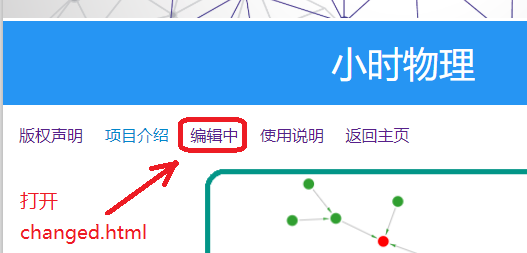
\includegraphics[width=9cm]{./figures/readme1.png}
\caption{查看编辑中的词条} \label{readme_fig1}
\end{figure}

每个词条文件(后缀名为 tex)都有一个独一无二的文件名, 可以将通过将光标停留在编辑器中的 tab 上查看.

\begin{figure}[ht]
\centering
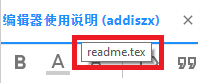
\includegraphics[width=5cm]{./figures/readme2.png}
\caption{查看编辑器中打开的词条的文件名} \label{readme_fig2}
\end{figure}

每个词条(section) 的 label 与文件名相同, 转换后输出的 html 文件也由相同的文件名, 可以在浏览器的地址栏中看到(例如本文的 tex 文件是 readme.tex, label 是 readme, 转换成网页为 readme.html).

\subsection{编辑器说明}
\begin{itemize}
\item 将光标停留在任意按钮上都会出现提示说明按钮的名称. 要新建词条, 点击红色的加号按钮, 根据提示新建即可. 要打开已有词条, 点击最右边的打开, 搜索需要的词条即可

\item 按下保存按钮(快捷键 \lstinline|Ctrl + s|) 会自动保存并编译

\item 如果要在 html 预览和 LaTex 代码之间跳转, 可以通过搜索关键词实现. 例如在预览窗口复制一段文字, 在编辑窗口搜索就可以跳转到对应内容

\item 要查看编辑器支持的所有命令和所有自定义的公式, 见 “词条示例(Sample)\upref{Sample}”. 当然, 所有已有的词条也都可以作为示例

\item 编辑器支持各种自动引用(被引用对象没有 label 时会自动插入 label), 工具栏上的内部引用按钮可以引用同一词条的公式, 图表, 例题等环境. 外部引用按钮可以引用其他词条的各种环境
\end{itemize}

\subsubsection{快捷键}

\begin{table}[ht]
\centering
\caption{请输入表格标题}\label{readme_tab1}
\begin{tabular}{|c|c|c|c|}
\hline
保存词条 & \lstinline|Ctrl + S| & 打开词条 & \lstinline|Ctrl + O| \\
\hline
新建词条 & \lstinline|Ctrl + Alt + N| & 关闭词条 & \lstinline|Ctrl + Alt + W| \\
\hline
显示编辑器选项 & \lstinline|Ctrl + Q| & 跳转到某行 & \lstinline|Ctrl + L| \\
\hline
查找文本 & \lstinline|Ctrl + F| & 替换文本 & \lstinline|Ctrl + H| \\
\hline
向左缩进 & \lstinline|Ctrl + [| & 向右缩进 & \lstinline|Ctrl + ]| \\
\hline
增大字号 & \lstinline|Shift + Alt + (+)| & 减小字号 & \lstinline|Shift + Alt + (-)| \\
\hline
关闭不保存 & \lstinline|Shift + 点关闭| &  &  \\
\hline
\end{tabular}
\end{table}

\subsection{公式}
\begin{itemize}
\item 公式环境支持大部分 LaTeX 命令, 严格来说是所有 \link{MathJax}{https://www.mathjax.org/} 支持的命令\footnote{MathJax 项目用于在网页上显示 LaTeX 公式}.
\item 支持部分 \link{Physics 宏包}{http://mirrors.ibiblio.org/CTAN/macros/latex/contrib/physics/physics.pdf}中的命令.
\item 我们把 \lstinline|\vec| 命令重新定义为正体和粗体, 如 \lstinline|\vec a| 被显示为 $\vec a$.
\end{itemize}

\subsection{格式要求}

\begin{itemize}
\item 行内公式用美元符号
\item 独立公式用 equation 环境, align 环境或者 gather 环境
\end{itemize}
